%% -*-TeX-*-
 % ###################################################################
 %  FiPy - a finite volume PDE solver in Python
 % 
 %  FILE: "fipy.tex"
 %                                    created: 4/1/04 {2:58:37 PM} 
 %                                last update: 7/30/04 {9:53:31 PM} 
 %  Author: Jonathan Guyer
 %  E-mail: guyer@nist.gov
 %  Author: Daniel Wheeler
 %  E-mail: daniel.wheeler@nist.gov
 %    mail: NIST
 %     www: http://ctcms.nist.gov
 %  
 % ========================================================================
 % This document was prepared at the National Institute of Standards
 % and Technology by employees of the Federal Government in the course
 % of their official duties.  Pursuant to title 17 Section 105 of the
 % United States Code this document is not subject to copyright
 % protection and is in the public domain.  fipy.tex
 % is an experimental work.  NIST assumes no responsibility whatsoever
 % for its use by other parties, and makes no guarantees, expressed
 % or implied, about its quality, reliability, or any other characteristic.
 % We would appreciate acknowledgement if the document is used.
 % 
 % This document can be redistributed and/or modified freely
 % provided that any derivative works bear some notice that they are
 % derived from it, and any modified versions bear some notice that
 % they have been modified.
 % ========================================================================
 % See the file "license.terms" for information on usage and  redistribution of
 % this file, and for a DISCLAIMER OF ALL WARRANTIES.
 %  
 % ###################################################################
 %%

\documentclass[letterpaper]{book}

\usepackage[text={7in,9.333in}]{geometry}

\usepackage{crop}

\usepackage{alltt, parskip, boxedminipage} % fancyheadings,  
\usepackage{multirow, longtable, makeidx, tocbibind, amssymb} 
\usepackage{amsmath} 

\usepackage{minitoc}
% \setcounter{tocdepth}{0}
\setcounter{parttocdepth}{1}

\usepackage[ascii]{inputenc}

%\usepackage{multirow, longtable, tocbibind, amssymb} % makeidx, 
% \usepackage{fullpage}
%\usepackage[headings]{fullpage}
\makeindex
\usepackage[usenames]{color}
\definecolor{darkblue}{rgb}{0,0.05,0.35}
\definecolor{redish}{rgb}{0.894,0.122,0.122}
\definecolor{bluish}{rgb}{0.216,0.188,0.533}
% \usepackage[dvips, pagebackref, pdftitle={FiPy}, pdfcreator={epydoc 2.1}, bookmarks=true, bookmarksopen=false, pdfpagemode=UseOutlines, colorlinks=true, linkcolor=black, anchorcolor=black, citecolor=black, filecolor=black, menucolor=black, pagecolor=black, urlcolor=darkblue]{hyperref}
\usepackage[urlcolor=blue,linkcolor=blue,bookmarksopen,bookmarksopenlevel=2,pdftex,pagebackref,pdftitle={FiPy}, pdfcreator={epydoc 2.1}, bookmarks=true, bookmarksopen=false, pdfpagemode=UseOutlines,colorlinks=true,plainpages=false,pdfpagelabels]{hyperref}
\usepackage{graphicx}
% \usepackage{memhfixc}
% \usepackage{nameref}

\graphicspath{{../figures/}}

% for reStructuredText
\usepackage{shortvrb}
\usepackage{tabularx}
\setlength{\extrarowheight}{2pt}
\newlength{\admonitionwidth}
\setlength{\admonitionwidth}{0.9\textwidth}
\newlength{\docinfowidth}
\setlength{\docinfowidth}{0.9\textwidth}
\newlength{\locallinewidth}
\newcommand{\optionlistlabel}[1]{\bf #1 \hfill}
\newenvironment{optionlist}[1]
{\begin{list}{}
  {\setlength{\labelwidth}{#1}
   \setlength{\rightmargin}{1cm}
   \setlength{\leftmargin}{\rightmargin}
   \addtolength{\leftmargin}{\labelwidth}
   \addtolength{\leftmargin}{\labelsep}
   \renewcommand{\makelabel}{\optionlistlabel}}
}{\end{list}}
% begin: floats for footnotes tweaking.
\setlength{\floatsep}{0.5em}
\setlength{\textfloatsep}{\fill}
\addtolength{\textfloatsep}{3em}
\renewcommand{\textfraction}{0.5}
\renewcommand{\topfraction}{0.5}
\renewcommand{\bottomfraction}{0.5}
\setcounter{totalnumber}{50}
\setcounter{topnumber}{50}
\setcounter{bottomnumber}{50}
% end floats for footnotes
% some commands, that could be overwritten in the style file.
\newcommand{\rubric}[1]{\subsection*{~\hfill {\it #1} \hfill ~}}
\newcommand{\titlereference}[1]{\textsl{#1}}


\newcommand{\logo}{\rotatebox{4}{\textcolor{redish}{\( \varphi \)}}\kern-.70em\raisebox{-.15em}{\textcolor{bluish}{\( \pi\)}}}
% \newcommand{\logoToo}{\raisebox{-.15em}{\textcolor{bluish}{\(\pi\)}}\kern-.64em\rotatebox{4}{\textcolor{redish}{\( \varphi \)}}}

\newcommand{\FiPy}{\textsf{FiPy}}

% \includeonly{installation}

\makeatletter
\renewcommand*\l@section{\@dottedtocline{1}{1.5em}{3.3em}}
\renewcommand*\l@subsection{\@dottedtocline{2}{3.8em}{4.2em}}
\renewcommand*\l@subsubsection{\@dottedtocline{3}{7.0em}{5.1em}}
\renewcommand*\l@paragraph{\@dottedtocline{4}{10em}{6em}}
\renewcommand*\l@subparagraph{\@dottedtocline{5}{12em}{7em}}

\renewcommand\tableofcontents{%
    \if@twocolumn
      \@restonecoltrue\onecolumn
    \else
      \@restonecolfalse
    \fi
    \chapter*{\contentsname\pdfbookmark[-1]{Contents}{contents}
        \@mkboth{%
           \MakeUppercase\contentsname}{\MakeUppercase\contentsname}}%
    \@starttoc{toc}%
    \if@restonecol\twocolumn\fi
    }

\renewcommand\maketitle{\begin{titlepage}%
\let\footnotesize\small
\let\footnoterule\relax
\let \footnote \thanks
\null\vfil
\vskip 20\p@
\begin{flushright}%
  {\Huge \@title \par}%
  \vskip 3em%
  {\large
   \lineskip .75em%
    \begin{tabular}[t]{r@{}}%
      \@author
    \end{tabular}\par}%
    \vskip 1.5em%
  {\large \@date \par}%       % Set date in \large size.
\end{flushright}\par
\@thanks
\vfil\null
\end{titlepage}%
\setcounter{footnote}{0}%
\global\let\thanks\relax
\global\let\maketitle\relax
\global\let\@thanks\@empty
\global\let\@author\@empty
\global\let\@date\@empty
\global\let\@title\@empty
\global\let\title\relax
\global\let\author\relax
\global\let\date\relax
\global\let\and\relax
}

\makeatother

% \usepackage{layout}


\usepackage{tocvsec2}

\input{version}

\begin{document}

\doparttoc

% \crop[frame,axes]

\frontmatter

% \layout

% \settypeblocksize{9in}{7in}{*}
% \setlrmargins{*}{*}{*}
% \setulmargins{*}{*}{*}

% \settrimmedsize{8.5in}{11in}{*}       % pi/2
% % \settypeblocksize{40\onelineskip}{*}{0.61803}  % golden ratio
% \settypeblocksize{33\onelineskip}{*}{0.61803}  % golden ratio
% \setlength{\trimtop}{0pt}
% \setlength{\trimedge}{\stockwidth}
% \addtolength{\trimedge}{-\paperwidth}
% \addtolength{\trimedge}{-1.5in}
% \setlrmargins{*}{*}{2}
% % \setlrmargins{*}{1in}{*}
% \setulmargins{5\onelineskip}{*}{*}
% \setheadfoot{3\onelineskip}{3\onelineskip}
% \setheaderspaces{\onelineskip}{*}{*}
% \setmarginnotes{17pt}{65pt}{\onelineskip}

% \checkandfixthelayout

% \fixpdflayout

% \setlength{\parindent}{0ex}
\setlength{\fboxrule}{2\fboxrule}
\newlength{\BCL} % base class length, for base trees.

% \pagestyle{Ruled}
\renewcommand{\sectionmark}[1]{\markboth{#1}{}}
\renewcommand{\subsectionmark}[1]{\markright{#1}}

\newenvironment{Ventry}[1]%
  {\begin{list}{}{%
    \renewcommand{\makelabel}[1]{\texttt{##1:}\hfil}%
    \settowidth{\labelwidth}{\texttt{#1:}}%
    \setlength{\leftmargin}{\labelsep}%
    \addtolength{\leftmargin}{\labelwidth}}}%
  {\end{list}}

\newsavebox{\NISTbox}
\sbox{\NISTbox}{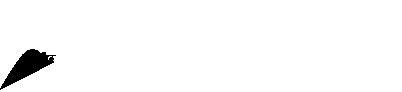
\includegraphics[trim=5 2 5 5,scale=1.5]{NIST_right2line}}
%\newlength{\photoheight}
%\settoheight{\photoheight}{\usebox{\photobox}}
%\newlength{\photowidth}
%\settowidth{\photowidth}{\usebox{\photobox}}

\makeatletter
\newcommand*{\ps@mytitlepage}{%
  \let\@oddhead\@empty
  \renewcommand*{\@oddfoot}{%
  \hfill\parbox[b][0pt]{0pt}{\makebox[0pt][r]{\usebox{\NISTbox}}}}}%\vspace*{-0.5in}}
\makeatother

\makeatletter  
\begin{titlepage}%
\thispagestyle{mytitlepage}
\let\footnotesize\small
\let\footnoterule\relax
\let \footnote \thanks
% \begin{flushleft}
%     \scalebox{10}{\logo}
% \end{flushleft}
% \null\vfil
% \vskip 20\p@
\begin{flushright}%
  \scalebox{10}{\logo}\par
%   \vspace*{\fill}
  \vskip 3em%
  {\Huge FiPy \\
    \huge A Finite Volume PDE Solver Using Python \par}%
  \vskip 3em%
  {\large
   \lineskip .75em%
    \begin{tabular}[t]{r@{}}%
        Daniel Wheeler \\
        Jonathan E. Guyer \\ 
        James A. Warren \\
        \textit{Metallurgy Division} \\
        \textit{Materials Science and Engineering Laboratory}
    \end{tabular}\par}%
    \vskip 1.5em%
  {\large \@date \par}%       % Set date in \large size.
      \vskip 1.5em%
  {\large Version~\Version \par}
% \vfil\null
  \vspace*{\fill}%
%   \raisebox{-5cm}{\fbox{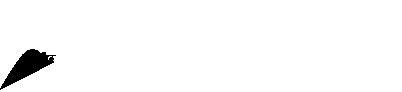
\includegraphics[hiresbb,scale=1.5]{NIST_right2line}}}%
\end{flushright}%
\end{titlepage}%
\makeatother

% \title{
% \scalebox{5}{\logo} \\[2ex]
% \Huge FiPy \\
% A Finite Volume PDE Solver Using Python \\
% }
% 
% \author{Daniel Wheeler, Jonathan E. Guyer \& James A. Warren \\
% Metallurgy Division, Materials Science and Engineering Laboratory\\
% National Institute of Standards and Technology}
% 
% \maketitle

\maxtocdepth{all} 
\tableofcontents
% \faketableofcontents

\mainmatter

\part{Introduction}

\settocdepth{chapter} 
\parttoc

\chapter{Installation}

\inputencoding{latin1}

\input installation

\inputencoding{ascii}

% \include{intro}

This chapter describes the numerical methods used to solve equations
in the \FiPy{} programming environment. \FiPy{} uses the finite volume
method (FVM) to solve coupled sets of partial differential equations
(PDEs). For a good introduction to the FVM see Nick Croft's PhD
thesis~\cite{croftphd}, Patanker~\cite{patanker} or Versteek and
Malalasekera~\cite{versteegMalalasekera}.

Essentially, the FVM consists of dividing the solution domain into
discrete finite volumes over which the state variables are
approximated with linear or higher order interpolations. The
derivatives in each term of the equation are satisfied with simple
approximate interpolations in a process known as discretization. The
(FVM) is a popular discretization technique employed to solve coupled
PDEs used in many application areas (\emph{e.g.} Fluid Dynamics).

The FVM can be thought of as a subset of the Finite Element Method
(FEM) as the Finite Difference Method (FDM) is a subset of the FVM. A
system of equations fully equivalent to the FVM can be obtained with
the FEM using as weighting functions the characteristic functions of
FV cells, i.e., functions equal to unity~\cite{mattiussi:1997}. Analogously,
the the discretization of equations with the FVM reduces to the FDM on
Cartesian grids.

\input numerical/equation
\input numerical/discret
\input numerical/scheme




\settocdepth{all} 

\part{Examples}

\settocdepth{chapter} 
\parttoc

\chapter{Diffusion Examples}

\input{examples/latex/examples.diffusion.steadyState.mesh1D.input-module}
\newpage
\input{examples/latex/examples.diffusion.steadyState.mesh1D.tri2Dinput-module}
\newpage
\input{examples/latex/examples.diffusion.steadyState.mesh20x20.input-module}
\newpage
\input{examples/latex/examples.diffusion.steadyState.mesh50x50.input-module}
\newpage
\input{examples/latex/examples.diffusion.explicit.mesh10.input-module}
\newpage
\input{examples/latex/examples.diffusion.explicit.mesh50.input-module}
\newpage
\input{examples/latex/examples.diffusion.variable.mesh2x1.input-module}
\newpage
\input{examples/latex/examples.diffusion.variable.mesh10x1.input-module}
\newpage
\input{examples/latex/examples.diffusion.variable.mesh50x1.input-module}
\newpage
\input{examples/latex/examples.diffusion.nthOrder.input2ndOrder1D-module}
\newpage
\input{examples/latex/examples.diffusion.nthOrder.input4thOrder1D-module}
\newpage

\chapter{Convection Examples}

\input{examples/latex/examples.convection.exponential1D.input-module}
\newpage
\input{examples/latex/examples.convection.exponential1DBack.input-module}
\newpage
\input{examples/latex/examples.convection.exponential1DSource.input-module}
\newpage
\input{examples/latex/examples.convection.exponential2D.input-module}
\newpage
\input{examples/latex/examples.convection.powerLaw1D.input-module}
\newpage

\chapter{Phase Field Examples}

\input{examples/latex/examples.phase.anisotropy.input-module}
\newpage
\input{examples/latex/examples.phase.impingement.mesh40x1.input-module}
\newpage
\input{examples/latex/examples.phase.impingement.mesh20x20.input-module}
\newpage
\input{examples/latex/examples.phase.impingement.restart.input-module}
\newpage
\input{examples/latex/examples.phase.missOrientation.circle.input-module}
\newpage
\input{examples/latex/examples.phase.missOrientation.mesh1D.input-module}
\newpage
\input{examples/latex/examples.phase.missOrientation.modCircle.input-module}
\newpage
\input{examples/latex/examples.phase.symmetry.input-module}
\newpage

\chapter{Level Set Examples}

\input{examples/latex/examples.levelSet.distanceFunction.oneD.input-module}
\newpage
\input{examples/latex/examples.levelSet.distanceFunction.square.input-module}
\newpage
\input{examples/latex/examples.levelSet.distanceFunction.circle.input-module}
\newpage
\input{examples/latex/examples.levelSet.distanceFunction.interior.input-module}
\newpage
\input{examples/latex/examples.levelSet.advection.mesh1D.input-module}
\newpage
\input{examples/latex/examples.levelSet.advection.circle.input-module}
\newpage

\chapter{Electrochemistry Phase Field Examples}

\input{examples/latex/examples.elphf.input1Dphase-module}
\newpage
\input{examples/latex/examples.elphf.input1D-module}
\newpage
\input{examples/latex/examples.elphf.input1Ddimensional-module}
\newpage
\input{examples/latex/examples.elphf.input2D-module}
\newpage
\input{examples/latex/examples.elphf.input2Dcorner-module}
\newpage
\input{examples/latex/examples.elphf.input1DpoissonAllCharge-module}
\newpage
\input{examples/latex/examples.elphf.input1DpoissonLeftCharge-module}
\newpage
\input{examples/latex/examples.elphf.input1DpoissonRightCharge-module}
\newpage
\input{examples/latex/examples.elphf.input1DphaseBinary-module}
\newpage
\input{examples/latex/examples.elphf.input1DphaseQuaternary-module}
\newpage
\input{examples/latex/examples.elphf.input1DphaseTernAndElectrons-module}
\newpage

\settocdepth{all} 

% \include{examples}
% 
% \include{theory}
% 
% \include{code}
 
\appendix

\part{APIs}

\settocdepth{chapter} 

\parttoc

\input api

\settocdepth{all} 

\backmatter

%%%%%%%%%%%%%%%%%%%%%%%%%%%%%%%%%%%%%%%%%%%%%%%%%%%%%%%%%%%%%%%%%%%%%%%%%%%
%%                                 Index                                 %%
%%%%%%%%%%%%%%%%%%%%%%%%%%%%%%%%%%%%%%%%%%%%%%%%%%%%%%%%%%%%%%%%%%%%%%%%%%%

% \pdfbookmark[-1]{Index}{index}
\printindex


\end{document}
